% !TeX root = ../main.tex

\section{Implementación del motor de optimización}
Este capítulo describe la materialización de la propuesta teórica en un artefacto de software funcional, detallando la arquitectura del sistema, las estructuras de datos seleccionadas para el manejo eficiente de memoria y el flujo de procesamiento de la información. La implementación, denominada \texttt{quickshift}, fue desarrollada en el lenguaje de sistemas Rust para garantizar la seguridad de memoria y minimizar la latencia de ejecución


\begin{figure}[H]
\centering
\begin{tikzpicture}[
  node distance=1.3cm,
  box/.style={rectangle, draw, align=center, rounded corners, minimum width=3cm, minimum height=1.0cm, fill=gray!10},
  arrow/.style={->, thick},
  every node/.style={font=\scriptsize}
]
\node[box, fill=blue!15]   (ingesta) {\textbf{1. Ingesta} \\ Excel + $\Phi(s)$};
\node[box, fill=purple!15, right=of ingesta] (pert) {\textbf{2. PERT} \\ Calcular $H$, $CC$};
\node[box, fill=green!15, right=of pert] (filtros) {\textbf{3. Filtros} \\ Prerreq. + Usuario};
\node[box, fill=yellow!15, below=of pert] (greedy) {\textbf{4. Greedy} \\ Multi-seed};
\node[box, fill=orange!15, right=of greedy] (json) {\textbf{5. Output} \\ JSON (Top 10)};

\draw[arrow] (ingesta) -- (pert);
\draw[arrow] (pert) -- (filtros);
\draw[arrow] (filtros) |- (greedy);
\draw[arrow] (greedy) -- (json);
\end{tikzpicture}
\caption{Pipeline del motor de optimización. Cada etapa reduce drásticamente el espacio de búsqueda antes de la construcción del horario.}
\\label{fig:pipeline_fase1}
\end{figure}

\subsection{Análisis de Ruta Crítica}

Se construye un DAG de correlatividades y se calcula la holgura total ($H$). Las asignaturas críticas ($H=0$) reciben un puntaje base mayor, pues retrasarlas afecta directamente el tiempo de titulación.

\subsection{Validación de prerrequisitos}

% Figura se mantiene
\begin{figure}[H]
\centering
\begin{tikzpicture}[
    node distance=1.5cm,
    decision/.style={diamond, draw, aspect=2, minimum width=2.5cm, minimum height=1.0cm, align=center, fill=yellow!10, font=\footnotesize},
    box/.style={rectangle, draw, rounded corners, minimum width=2.5cm, minimum height=0.8cm, align=center, font=\footnotesize},
    arrow/.style={->, thick},
]
\node[box, fill=blue!10] (input) {Asignatura Candidata $A$};
\node[decision, below=of input] (hasreq) {¿Tiene prerrequisitos?};
\node[box, left=1cm of hasreq, fill=green!10] (valid1) {\textbf{Válida} \\ Sin prereq.};
\node[decision, below=of hasreq] (check) {¿Todos están \\ en aprobados?};
\node[box, right=1cm of check, fill=red!10] (invalid) {\textbf{Descartar}};
\node[box, below=of check, fill=green!10] (valid2) {\textbf{Válida}};

\draw[arrow] (input) -- (hasreq);
\draw[arrow] (hasreq) -- node[above] {No} (valid1);
\draw[arrow] (hasreq) -- node[right] {Sí} (check);
\draw[arrow] (check) -- node[above] {No} (invalid);
\draw[arrow] (check) -- node[right] {Sí} (valid2);
\end{tikzpicture}
\caption{Árbol de decisión para la validación de prerrequisitos.}
\end{figure}

\subsection{Función de Prioridad}

La prioridad total de una sección se define como:

\[
P = CC \cdot 10^6 + UU \cdot 10^4 + KK \cdot 10^2 + SS.
\]

Este puntaje permite ordenar las secciones para guiar la estrategia greedy.

\subsection{Construcción de cliques}


El motor realiza una combinación de análisis estructural (PERT), filtrado académico, evaluación de preferencias y construcción de cliques compatibles. El flujo completo se muestra en la Figura \ref{fig:pipeline_fase1}.

% Pipeline (idéntico, con mejor explicación en caption)
\begin{figure}[H]
\centering
\begin{tikzpicture}[
  node distance=1.3cm,
  box/.style={rectangle, draw, align=center, rounded corners, minimum width=3cm, minimum height=1.0cm, fill=gray!10},
  arrow/.style={->, thick},
  every node/.style={font=\scriptsize}
]
\node[box, fill=blue!15]   (ingesta) {\textbf{1. Ingesta} \\ Excel + $\Phi(s)$};
\node[box, fill=purple!15, right=of ingesta] (pert) {\textbf{2. PERT} \\ Calcular $H$, $CC$};
\node[box, fill=green!15, right=of pert] (filtros) {\textbf{3. Filtros} \\ Prerreq. + Usuario};
\node[box, fill=yellow!15, below=of pert] (greedy) {\textbf{4. Greedy} \\ Multi-seed};
\node[box, fill=orange!15, right=of greedy] (json) {\textbf{5. Output} \\ JSON (Top 10)};

\draw[arrow] (ingesta) -- (pert);
\draw[arrow] (pert) -- (filtros);
\draw[arrow] (filtros) |- (greedy);
\draw[arrow] (greedy) -- (json);
\end{tikzpicture}
\caption{Pipeline del motor de optimización. Cada etapa reduce drásticamente el espacio de búsqueda antes de la construcción del horario.}
\label{fig:pipeline_fase2}
\end{figure}



La generación de horarios se modela como la construcción de un \textit{clique} compatible. Para evitar el costo de construir una matriz de adyacencia ($O(N^2)$), \texttt{quickshift} verifica compatibilidades \textit{on-the-fly}.

% Figura mejorada se mantiene
\begin{figure}[H]
\centering
\begin{tikzpicture}[
    node distance=1.0cm,
    every node/.style={font=\footnotesize},
    box/.style={rectangle, draw, rounded corners, minimum width=6cm, minimum height=0.7cm, align=left, fill=gray!5},
    seed/.style={rectangle, draw, rounded corners, minimum width=6cm, minimum height=0.7cm, align=left, fill=yellow!15, thick},
    added/.style={rectangle, draw, rounded corners, minimum width=6cm, minimum height=0.7cm, align=left, fill=green!15},
    rejected/.style={rectangle, draw, rounded corners, minimum width=6cm, minimum height=0.7cm, align=left, fill=red!10},
    arrow/.style={->, thick, >=stealth}
]

\node[box, fill=blue!10, align=center] (lista) {\textbf{Candidatos ordenados} \\ \texttt{[S1, S2, S3, S4]}};
\node[seed, below=0.8cm of lista] (step1) {\textbf{Seed: S1} \\ \texttt{Clique = \{S1\}}};
\draw[arrow] (lista) -- (step1);

\node[added, below=0.6cm of step1] (step2) {\textbf{Incorporar S2} \\ Compatible con S1};
\draw[arrow] (step1) -- (step2);

\node[added, below=0.6cm of step2] (step3) {\textbf{Incorporar S3} \\ Compatible con S1 y S2};
\draw[arrow] (step2) -- (step3);

\node[rejected, below=0.6cm of step3] (step4) {\textbf{Rechazar S4} \\ Incompatibilidad horaria};
\draw[arrow] (step3) -- (step4);

\node[box, below=0.6cm of step4, fill=orange!15, align=center] (final) {\textbf{Clique final:} \{S1, S2, S3\}};
\draw[arrow] (step4) -- (final);

\end{tikzpicture}
\caption{Proceso de expansión greedy para la construcción de un horario válido.}
\end{figure}


\section{Resultados experimentales}

El sistema fue evaluado sobre 692 secciones reales. La mejora obtenida se resume en la Figura \ref{fig:benchmark} y en la Tabla \ref{tab:metricas_implementacion}.

% Figura de benchmark igual
\begin{figure}[H]
\centering
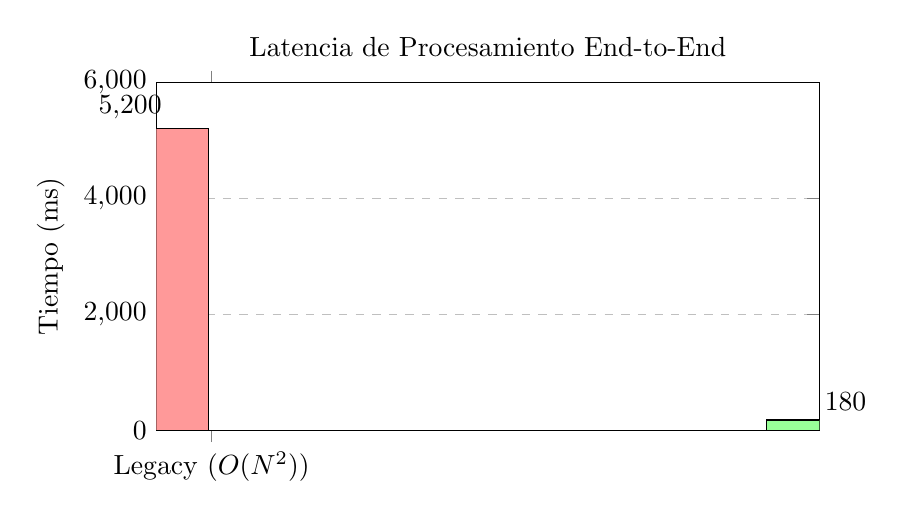
\begin{tikzpicture}
    \begin{axis}[
        ybar,
        symbolic x coords={Legacy ($O(N^2)$), Quickshift ($O(N)$)},
        xtick=data,
        ylabel={Tiempo (ms)},
        ymin=0,
        ymax=6000,
        nodes near coords,
        bar width=2cm,
        width=10cm,
        height=6cm,
        title={Latencia de Procesamiento End-to-End},
        ymajorgrids=true,
        grid style=dashed,
    ]
    \addplot[fill=red!40] coordinates {(Legacy ($O(N^2)$),5200)};
    \addplot[fill=green!40] coordinates {(Quickshift ($O(N)$),180)};
    \end{axis}
\end{tikzpicture}
\caption{Comparación de tiempos entre el sistema legado y la versión optimizada.}
\label{fig:benchmark}
\end{figure}

% Tabla igual pero corregida semánticamente
\begin{table}[H]
\centering
\caption{Impacto de la optimización en métricas operativas.}
\label{tab:metricas_implementacion}
\begin{tabular}{@{}lcc@{}}
\toprule
\textbf{Indicador} & \textbf{Sistema Legado} & \textbf{Quickshift} \\ \midrule
Horarios generados & 0 & $\approx 600$ \\
Cobertura efectiva & 0\% & 87\% \\
Tiempo de respuesta & $>5000$ ms & $<200$ ms \\
Validación académica & Parcial & Completa \\ \bottomrule
\end{tabular}
\end{table}

